%!TEX root = ../../main.tex
\chapter{序論}
\label{chap:intro}

\section{本研究の背景}
本システムでは,まずはケーススタディとして大学の研究室を対象とする.
学生の研究目標を公開・共有することによって,教員による進捗の把握や,学生の自律性向上,学生同士の協働の促進を目的としている.
また作成されたデータは後から一般公開できるので,外部組織との連携やアウトリーチ活動にも活用でき,これまでのゴオルシェアが対象とするような公益活動にも研究シーズを活用できる可能性がある.
初期段階では本研究室内で試用し,有用性を検証する.

\section{本研究の目的}
組織を超えた協働プロジェクトを円滑に進行させるには,(1)プロジェクト全体のタスクを俯瞰できる,(2)後から参加した人でも議論に参加しやすいような議事録作り,(3)誰が何をどこまでやったのかが把握できる進捗管理,という3つの要件を満たす必要がある.
このような要件を満たすシステムは”プロジェクト管理システム”と呼ばれ,有償無償問わず数多く存在する.
上記のような従来型のプロジェクト管理システムの機能に加え,プロジェクトの成果を公開することで,2次活用や外部組織との連携に役立てられることができれば,新たな協働を生む可能性がある.
そこで新システムMissionForestの試作により,新たな協働を生み,協働を支援できるようなプロジェクト管理システムを目指す.
プロジェクトの目標階層は,ゴオルシェアを踏襲してLinked Dataとして構造化した上で,ゴオルシェアよりも詳細に公開/非公開を制御できる機構を目指す.

\subsection{システム構成}
本システムのシステム構成を図\ref{img:system_architecture}に示す.
ユーザーの認証情報やミッションのすべての情報は,まずはメインDBに保存される.次に,タスクごとに設定されたアクセス権限により,LODとしてRDFストアにコピーされる.
\begin{figure}[t]
	\begin{center}
		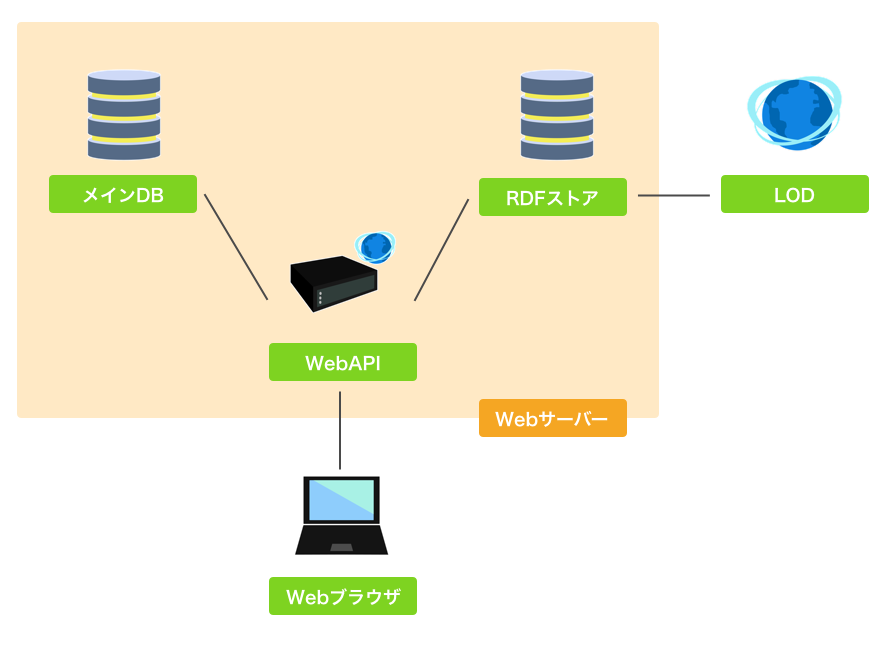
\includegraphics[width=0.9\linewidth]{assets/img/system_architecture.png}
		\caption{システム構成図}
		\label{img:system_architecture}
	\end{center}
\end{figure}

\section{本論文の構成}
本論文の構成を以下に示す.
第2章では関連研究や関連システムと本研究の動作・開発環境について述べる.
第3章では直感的にツリーを作成できるインターフェースについて述べる.
第4章ではLODでの公開機構について述べる.
第5章では類似タスクの推薦機構について述べる.
第6章では前章までで述べたシステムの評価実験の結果をまとめる.
第7章で本研究をまとめる.
